Each of the radionuclide contaminant transport models described in Section
\ref{sec:nuclide_models} capture different combintations of physics present in
the hydrologic contaminant transport problem. To determine how effectively
these physics were captured, single-effect simulations were conducted with
\Cyder and compared to analysis was conducted with a more detailed radionuclide
transport model, the Clay \gls{GDSM} \cite{clayton_generic_2011}. The Clay
\gls{GDSM} was developed by the \gls{UFD} Campaign within the \gls{DOE} Office
of Nuclear Energy and relies on the GoldSim simulation environment
\cite{golder_associates_goldsim_2010} and its contaminant transport module
\cite{golder_associates_goldsim_2010-1}.

These single-effect sensitivity analyses were constructed by repeated
multi-component simulation runs conducted accross the valid range for a single
parameter.

To verify the behavior of the solubility limitation model in the Mixed Cell
model, for example, one hundred multi-component simulations were conducted,
each with a different reference solubility limit. This parametric analysis was
conducted to show that, for an arbitrary isotope, the expected solubility
limitation behavior is captured. In the case of real isotopes in a full
simulation, the same model will be invoked with real parameters for each
isotope. Thus, the this model agreement is representative in all cases.

The results acheived with \Cyder were compared to the results of a parametric
sensitivity analysis using the Clay \gls{GDSM} reported in
\cite{huff_key_2012}. That analysis showed that for solubility limits below a
certain threshold, the dose releases were directly proportional to the
solubility limit, indicating that the radionuclide concentration saturated the
groundwater up to the solubility limit near the waste form.  For solubility
limits above the threshold, however, further increase to the limit had no
effect on the peak dose. This demonstrates the situation in which the
solubility limit is so high that even complete dissolution of the waste
inventory into the pore water is insufficient to reach the solubility limit.

\begin{figure}[ht]
\begin{center}
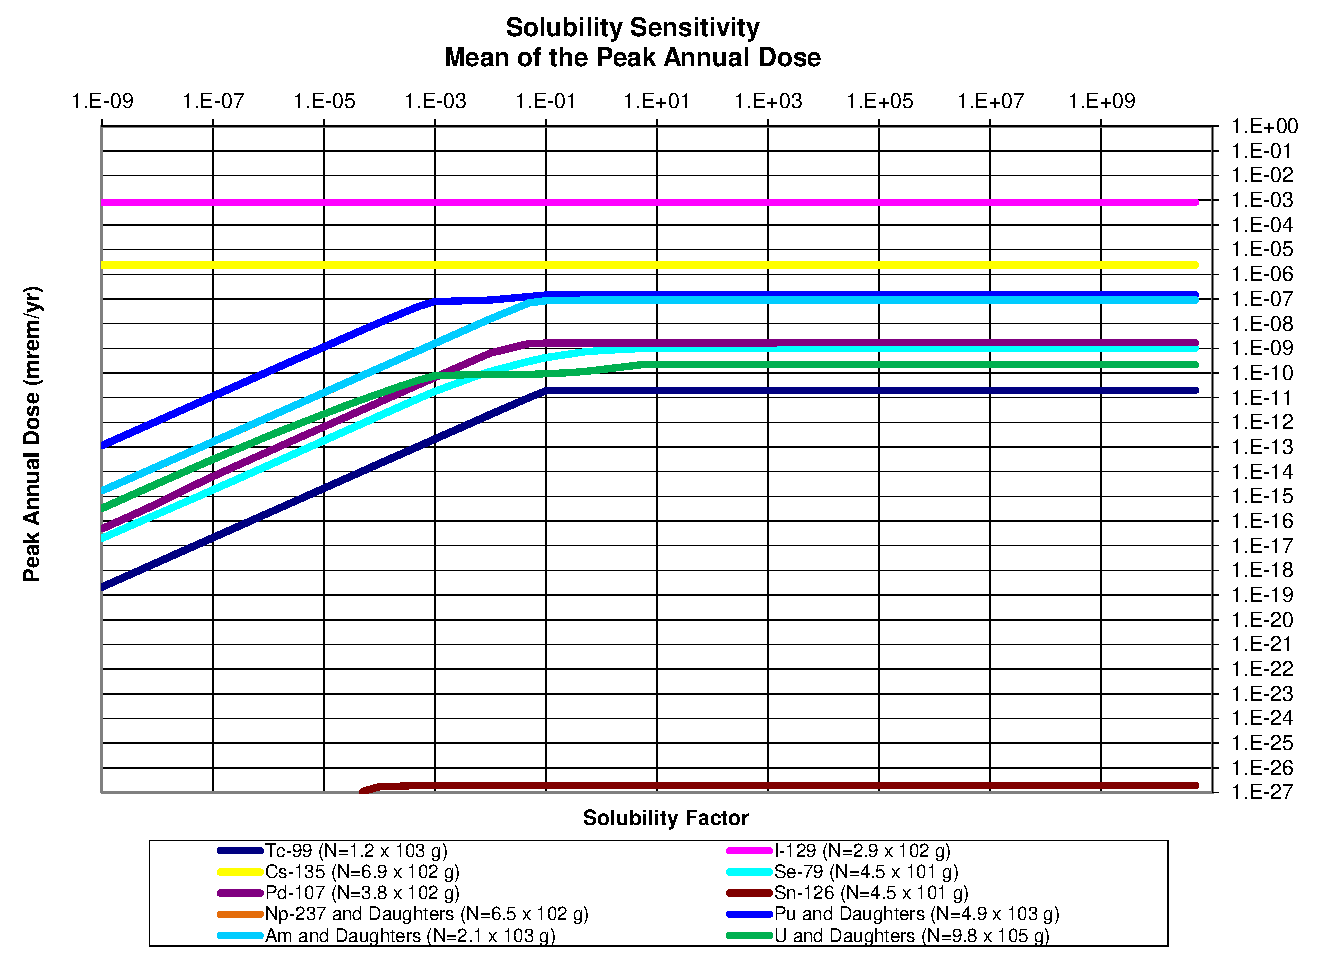
\includegraphics[width=0.7\linewidth]{./Solubility_Summary_SolFactor.eps}
\caption[Solubility factor sensitivity in GDSM Clay model]{Solubility factor sensitivity. The peak annual dose due to an inventory, $N$, of each isotope. This result was acheived with a parametric analysis using a detailed model of a generic clay repository \ref{huff_key_2012}}
\label{fig:SolSumFactor}
\end{center}
\end{figure}

\begin{figure}[ht]
\begin{center}
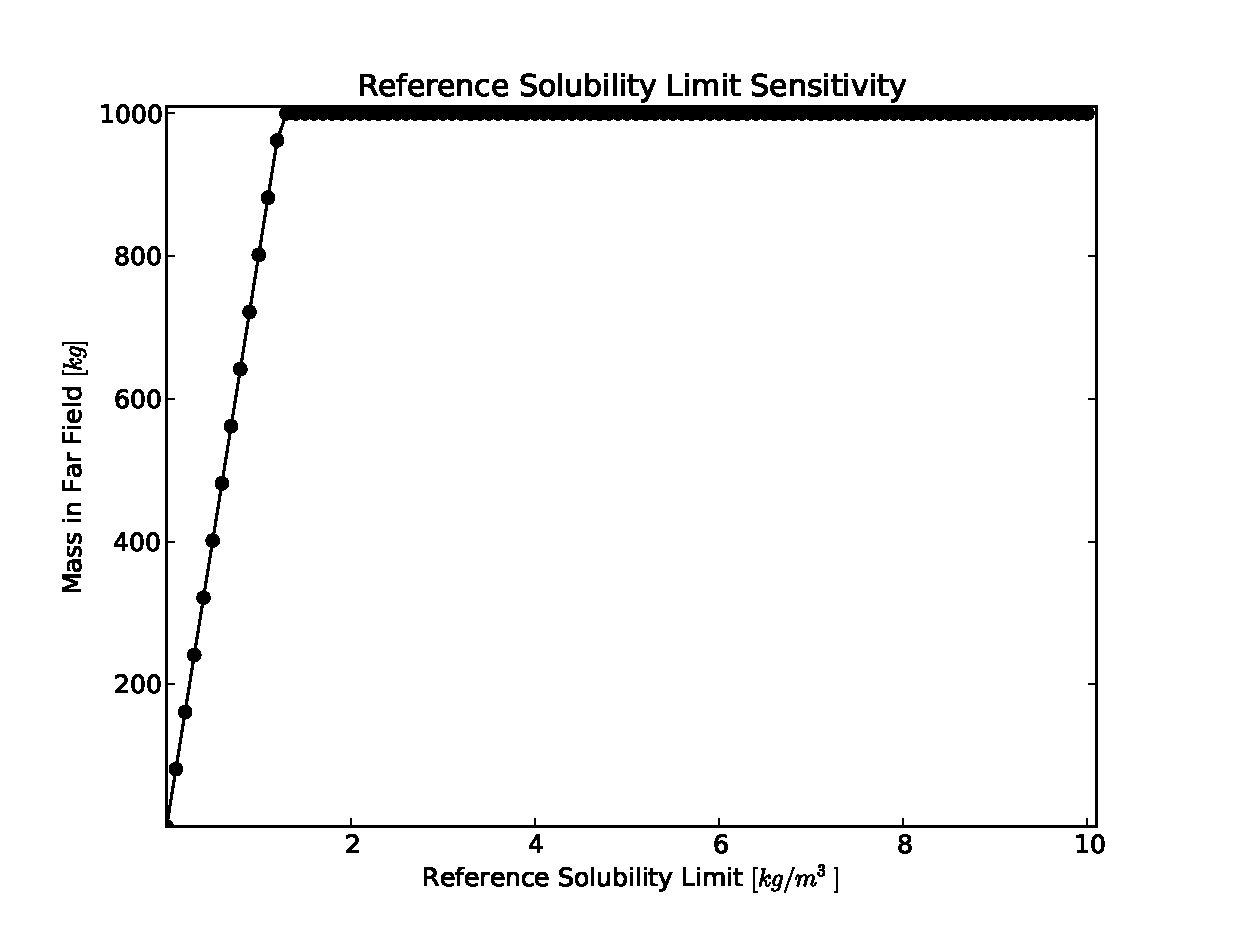
\includegraphics[width=0.7\linewidth]{./sol.eps}
\caption[Solubility Sensitivity in the Mixed Cell Model]{Sensitivity demonstration of solubility limitation in \Cyder for an arbitrary isotope assigned a variable solubility limit.}
\label{fig:sol_result}
\end{center}
\end{figure}


The results in Figure \ref{fig:SolSumFactor}, from the detailed parametric
analysis in \cite{huff_key_2012}, it is clear that for
solubility constants lower than the saturation threshold, the transport regime is solubility
limited and the relationship between peak annual dose and solubility limit is
strong.  Above the threshold, the transport regime is inventory limited
instead.

In the corresponding parametric analysis of \Cyder performance, it was shown that the
solubility sensitivity behavior closely matched that of the \gls{GDSM}
sensitivity behaviors. Specifically, in Figure \ref{fig:sol_result}, a sharp turnover
is seen where the solubility limit exceeds the point at which it limits
movement. For increased solubility limits, release remains constant, as
expected.

%\begin{figure}[ht]
%\begin{center}
%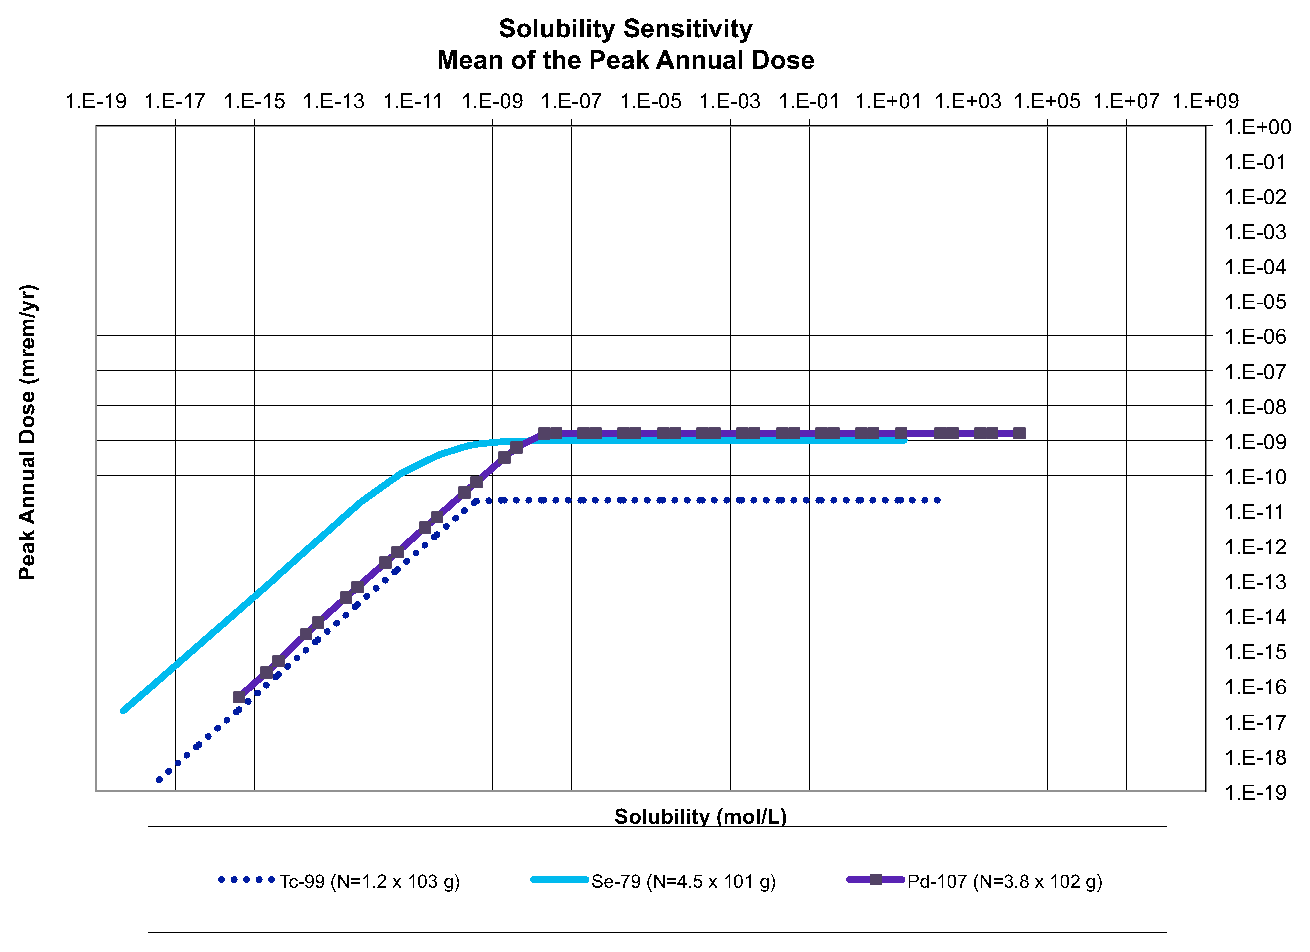
\includegraphics[width=0.7\linewidth]{./Solubility_Summary_Sol.eps}
%\caption[Solubility limit sensitivity in GDSM Clay model]{Solubility limit sensitivity. The peak annual dose due to an inventory,
%$N$, of each isotope.}
%\label{fig:SolSum}
%\end{center}
%\end{figure}

